Observamos que el hamiltoniano \eqref{eq:k_space_capacitive_hamiltonian} en ausencia del término Kerr es cuadrático en los operadores $\hat b^\dag$, $\hat b$ por lo cual formalmente puede ser diagonalizado por una transformación de Bogoliubov \cite{vanHemmen1980}. Sin embargo es ilustrativo realizar el proceso de diagonalización paso a paso. Primero realizamos un cambio de gauge 
\begin{subequations}
    \begin{align}
        \hat b_{kA} &\rightarrow e^{i\varphi_A(k)}\hat b_{kA}\\
        \hat b_{kB} &\rightarrow e^{i\varphi_B(k)}\hat b_{kB}
    \end{align}\label{eq:first_gauge}
\end{subequations}
Del cual se puede mostrar (ver apéndice \ref{appendix:diagonalization}) que lo más conveniente es tomar un gauge impar $\varphi_\sigma(-k) = - \varphi_\sigma(k)$ y a su vez $\varphi_B(k) - \varphi_A(k) = \operatorname{Arg}(\Delta_C(k))$. De esta manera 
\begin{subequations}
    \begin{align}
        \Delta_C(k)&\rightarrow \abs{\Delta_C(k)}\\
        \Delta_J(k)&\rightarrow \Delta_J(k)e^{-i\operatorname{Arg}(\Delta_C(k))}
    \end{align}
\end{subequations}
Luego explotamos la simetría de intercambio de subred que tiene $H_C$ en este gauge observando que $\left[\hat H_C, \mathcal I\right] = \left[\hat H_C, \mathcal T\right] = \left[\mathcal I, \mathcal T\right] =  0$ con 
\begin{subequations}
    \begin{align}
        \mathcal I : \hat b_{kA} \leftrightarrow \hat b_{kB}\\
        \mathcal T: \hat b_{k\sigma} \leftrightarrow \hat b_{-k\sigma}
    \end{align}\label{eq:symmetries}
\end{subequations}
que vendrían a ser las simetrías de inversión espacial y temporal respectivamente. Por tanto, el hamiltoniano tiene un grupo de simetría $\mathbb Z_2 \times \mathbb Z_2$. De esta forma, definimos los operadores de diagonalizan dichas operaciones de simetría, para $k > 0$:
\begin{subequations}
    \begin{align}
        \hat \alpha_{k} = \frac{1}{2}\left(\hat b_{kA} + \hat b_{kB} + \hat b_{-kA} + \hat b_{-kB}\right)\\
        \hat \alpha_{-k} = \frac{1}{2}\left(\hat b_{kA} + \hat b_{kB} - \hat b_{-kA} - \hat b_{-kB}\right)\\
        \hat \beta_{-k} = \frac{1}{2}\left(\hat b_{kA} - \hat b_{kB} + \hat b_{-kA} - \hat b_{-kB}\right)\\
        \hat \beta_{k} = \frac{1}{2}\left(\hat b_{kA} - \hat b_{kB} - \hat b_{-kA} + \hat b_{-kB}\right).
    \end{align}
\end{subequations}
Mientras que para $k = 0, -\pi$, los momentos invariantes ante inversión temporal (TRIMs):
\begin{subequations}
    \begin{align}
        \hat \alpha_{k} = \frac{1}{\sqrt{2}}\left(\hat b_{kA} + \hat b_{kB}\right)\\
        \hat \beta_{k} = \frac{1}{\sqrt{2}}\left(\hat b_{kA} - \hat b_{kB}\right).
    \end{align}
\end{subequations}
Para simplificar la notación definimos $\hat \eta_{k+} \equiv \hat \alpha_k$, $\hat \eta_{k-} \equiv \hat \beta_k$. En el apéndice se detalla el proceso completo de diagonalización, el cual en algún punto requiere hacer múltiples transformaciones squeeze $S_{k\sigma}$ por cada modo $k_\sigma$
 
\begin{subequations}
    \begin{align}
        \hat S^\dag \hat H_C \hat S &= \sum_{k\sigma} E_{k\sigma}\hat \eta_{k\sigma}^\dag \hat \eta_{k\sigma} + E_{\text{GS}}\\
        \hat S^\dag \hat H_J \hat S &= \sum_{k,\sigma}
                \epsilon^J_{k\sigma} \hat c^\dag_{k\sigma}\hat c_{k\sigma} 
                - \frac{\Delta^J_{k\sigma}}{2}\left((\hat c^\dag_{k\sigma})^2 + \text{h.c.}\right) \nonumber\\
               &\quad +\sum_{k}\left(t^J_k\hat c^\dag_{kA} \hat c_{kB} +\Delta^J_k\hat c^\dag_{kA}\hat c_{kB}^\dag+ \text{h.c.}\right) + \delta_{J}'\\
        \hat S &= \prod_{k\sigma} \hat S_{k\sigma}(z_{k\sigma})
    \end{align} \label{eq:squeeze_transform_total}
\end{subequations}
Para diagonalizar el hamiltoniano capacitivo requerimos 
\begin{align}
    \tanh(2z_{k\sigma}) 
        &= \frac{-\mathrm{sgn}(k)\,|\Delta_C(k)|}
               {\hbar\omega_q \pm |\Delta_C(k)|} \nonumber\\
    z_{k\sigma} 
        &= \frac{\mp\,\mathrm{sgn}(k)}{4}
           \ln\!\left(1 \pm \frac{|\Delta_C(k)|}{\hbar\omega_q}\right).
           \label{eq:squeeze_parameter}
\end{align}
La fórmula \eqref{eq:squeeze_parameter} aplica también para los TRIMs con la particularidad de tomar $\operatorname{Sgn}(k) = +1$ para ambos. Esta última es una pauta que se puede utilizar para el resto de fórmulas que dependen del símbolo de $\operatorname{Sgn}(k)$. Por otra parte, aplicando esta transformación, encontramos que las energías de transición de los modos bosónicos y la energía del estado base de $\hat H_C$ están dados por
\begin{subequations}
    \begin{align}
        E_{k\pm} &= \sqrt{\varepsilon_{k\pm}^2 - \Delta_{k\pm}^2}\nonumber\\
        &= \hbar \omega_q \sqrt{1 \pm \frac{2\abs{\Delta_C(k)}}{\hbar \omega_q}}\\
        E_{\text{GS}} &= \frac{1}{2}\sum_{k\sigma}E_{k\sigma} - \varepsilon_{k\sigma} = \frac{1}{2}\sum_{k\sigma}E_{k\sigma} - N \hbar \omega_q
    \end{align}
\end{subequations}
Por lo general, soltamos este término de la energía del nuevo fundamental redefiniendo una nueva energía de vacío. A su vez, es posible soltar el término $\delta_J'$ en el límite de acoplamiento lineal $\gamma \ll 1$, ya que se lo puede quitar aplicando un operador desplazamiento $\hat D(\alpha) = \exp(\alpha \hat a^\dag - \alpha^*\hat a)$ sobre el fotón nuevamente renormalizando la energía del vacío. Los coeficientes exactos del hamiltoniano $\hat H_J$ se dejan en el apéndice. Para caracterizar el espectro, hacemos la siguiente parametrización
\begin{subequations}
    \begin{align}
        g_{C,1} + g_{C,2} &= 2g_C\\
        g_{C,1} - g_{C,2} &= 2\chi_C g_C 
    \end{align}\label{eq:coupling_auxiliary_variables}
\end{subequations}
con $-1\leq \chi_C \leq 1$. En la figura \ref{fig:capacitive_spectra} se muestran las bandas que surgen para distintas elecciones de $2g_C / \hbar \omega_q$ y de $\eta_C$ además de incluir el efecto del término Kerr en las bandas. Este último puede ser encontrado usando teoría de perturbaciones de primer orden (ver apéndice). Lo primero que se puede apreciar es que las bandas que se forman son asimétricas alrededor de la frecuencia propia del qubit $\hbar \omega_q$ y que esta asimetría aumenta conforme $2g_C \rightarrow \hbar \omega_C / 2$ y de hecho en este límite el modo $k = 0$ se ablanda y se vuelve \textit{gapless}. En el límite de acople capacitivo débil, se puede aproximar $4\frac{g_C}{\omega_q} = \frac{C_{g}}{C}$ siendo $C_g$ la capacitancia de acoplamiento y $C$ la capacitancia de shunt de cada transmon. Sin embargo, usando la expresión correcta, se encuentra que $4\frac{g_C}{\omega_q} = \frac{C_{g}}{C + 2C_{g}}$ por lo cual este límite requiere $\frac{C_g}{C}\rightarrow \infty$.
\begin{figure*}[t]
    \centering
    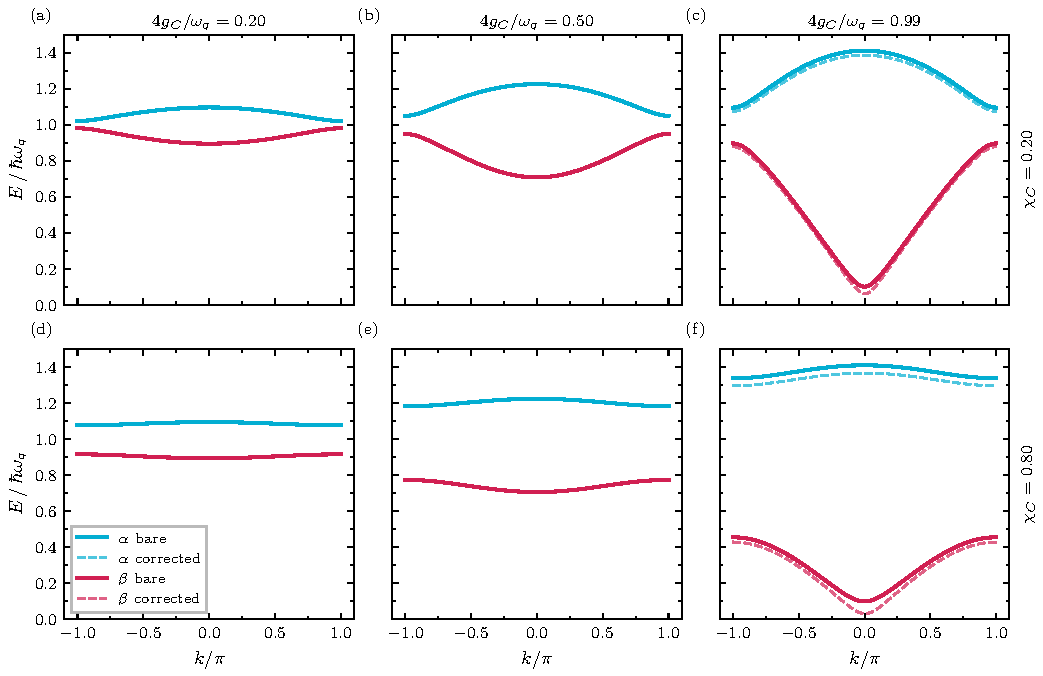
\includegraphics[width=\textwidth]{figures/ssh_chain_spectrum.pdf}
    \caption{
        relación de dispersión de las bandas $\alpha$ y $\beta$ con y sin correcciones del término Kerr a primer orden en perturbaciones. Las columnas corresponden a aumentar la magnitud de acoplamiento $4g_C/\omega_q$ y las filas la dimerización $\chi_C$. Las líneas continuas muestran la dispersión desnuda y las líneas discontinuas la dispersión corregida.
    }
    \label{fig:capacitive_spectra}
\end{figure*}
Se aprecia que, al igual que en la cadena SSH típica, el parámetro $\chi_C$ a $g_C$ fijo cambia la amplitud del gap. Por otra parte, $g_C$ manteniendo $\chi_C$ fijo no solo cambia el ancho de bandas sino que cambia la asimetría entre ellas y a su vez magnifica el efecto de las interacciones. Este último hecho se puede demostrar al calcular el número de excitaciones en la cadena cuando hay una excitación tipo $k\sigma$:
\begin{align}
    \hat N_{k\sigma} &\equiv \bra{\mathbf \Omega}\hat \eta_{k\sigma}\hat S^\dag \left(\sum_{j}\hat b^\dag_j \hat b_j \right)\hat S \hat \eta_{k\sigma}^\dag\ket{\mathbf{\Omega}}\nonumber\\
    &= \frac{\varepsilon_{k\sigma}}{E_{k\sigma}} + \underbrace{\frac{1}{2}\sum_{k'\sigma'}\frac{\varepsilon_{k'\sigma'}}{E_{k'\sigma'}} - 1}_{\bra{\mathbf{\Omega}}\hat N \ket{\mathbf{\Omega}}} \label{eq:excitation_number}
\end{align}
siendo $\ket{\mathbf{\Omega}}$ el nuevo vacío definido por la transformación squeeze. De \eqref{eq:excitation_number}, se ve que conforme $E_{k\sigma} \rightarrow 0$, el número de excitaciones en el sistema diverge y la descripción del estado $\eta_{k\sigma}^\dag \ket{\mathbf{\Omega}}$ requiere de un mayor número de excitaciones en cada qubit. Por este motivo es que también la renormalización de las bandas por el efecto Kerr toma mayor efecto en este límite: los estados son combinaciones lineales de niveles con mayores excitciones que tienen mayor efecto por parte del término Kerr. (Hot take) Consideramos (yo) que este fenómeno se debe a una ruptura progresiva del régimen transmon y que la descripción correcta del dispositivo requiere bien la inclusión de más ordenes del potencial o bien un análisis en la base de carga. Esto más adelante lo exploramos por medio de un análisis semiclásico de la dinámica de fases en la cadena para este límite.

\subsection{Adimensionalización del Hamiltoniano}
Para facilitar posteriores tratamientos, introducimos un conjunto de parámetros adimensionales. Al igual que hicimos con los acoplamientos capacitivos, hacemos la siguiente parametrización de los acoplamientos Josephson
\begin{subequations}
    \begin{align}
        g_{J,1} + g_{J,2} &= 2g_J \chi_J\\
        g_{J,1} - g_{J,2} &= 2g_J 
    \end{align}\label{eq:josephson_parametrization}
\end{subequations}
con $-1 \leq \chi_J \leq 1$ anticipando que $\operatorname{Sgn}(g_{J,2}) = - \operatorname{Sgn}(g_{J,1})$. Por otra parte, introducimos la siguiente función que caracteriza la geometría de la relación de dispersión
\begin{equation}
    \zeta_C(k) \equiv \sqrt{\chi_C^2 + (1-\chi_C^2) \cos^2(\frac{k}{2})}. 
\end{equation}
A su vez introducimos parámetros que caracterizan la intensidad de acoplamiento 
\begin{subequations}
    \begin{align}
        \Omega_C &\equiv \frac{4g_C}{\omega_q}\\
        \Omega_J &\equiv \frac{\gamma g_J}{\omega_q}
    \end{align}
\end{subequations}
Donde consideramos $0 < \Omega_C \leq 1$ y $\Omega_J > 0$. Finalmente midiendo la frecuencia del resonador $\omega_c$ en unidades de la frecuencia de transición de los transmon $\omega_q$, $\hat H / \hbar \omega_q$ tiene expresiones iguales a $\eqref{eq:squeeze_transform_total}$ para $\hat S^\dag \hat H_C \hat S$ y $\hat S^\dag \hat H_J \hat S$ pero con coeficientes dados por los nuevos parámetros adimensionales. En la tabla \ref{tab:parametros_chij_cero} presentamos los parámetros especializando al caso $\chi_J = 0$, en el apéndice presentamos las expresiones para un valor arbitrario de $\chi_J$. En este caso, observamos que los coeficientes longitudinales $\epsilon_{k\sigma}^J$, $\Delta_{k\sigma}^J$ dependen directamente de la dimerización $\chi_C$ por lo cual si esta se mantiene pequeña podemos despreciarlos. En la figura \ref{fig:josephson_coeffs} se presentan estos coeficientes para $\chi_J = 0$ para distintas elecciones de $\chi_C$ y $\Omega_C$. De esta figura se puede apreciar que $\chi_C$ juega un rol más importante que $\Omega_C$ a la hora de determinar el peso de los coeficientes de mezcla $t_k$, $\Delta_k$ sobre el resto. Además se aprecia que $\hat H_J$ se anula para $k = 0$ y que en $k=\pm \pi$ no hay mezcla entre los modos $\alpha$ y $\beta$. De esto se deduce que el diseño del dispositivo debe tener 3 o más celdas unidad para tener mezcla entre los modos $\alpha$ y $\beta$. Para resguardarse de efectos de decoherencia masivos, es favorable mantener el número de celdas unidad lo más pequeño posible en el dispositivo por lo cual determinamos usar 3 celdas unidad (6 qubits). Por otro lado, se ve que para que los términos de mezcla dominen sobre el resto en $k=\pm 2\pi/3$ es favorable una débil dimerización .
\begin{table}[h]
\centering
\caption{Parámetros adimensionalizados de $\hat H_J$ los símbolos superiores corresponden a los coeficientes para los modos $\alpha_k$ y los inferiores para los modos $\beta_k$.}
\label{tab:parametros_especializados}
\begin{ruledtabular}
\begin{tabular}{l|c}
Parámetro & $\hat S^\dag\hat H_J \hat S / \hbar \omega_q$ \\
\hline
$\epsilon^J_{k\sigma}$ &  $\mp \Omega_J \chi_C(1\pm \Omega_C \zeta_C(k))^{1/2} \cdot \frac{1-\cos k}{\zeta_C(k)}$ \\
$\Delta^J_{k\sigma}$ &  $\mp \operatorname{Sgn}(k)\Omega_J \chi_C (1\pm \Omega_C\zeta_C(k))^{1/2}\cdot \frac{1-\cos k}{\zeta_C(k)}$ \\
$t^J_k$ & $\Omega_J \frac{\abs{\sin k}}{\zeta_C(k)}\sqrt[4]{1-(\Omega_C \zeta_C(k))^2}$ \\
$\Delta^J_k$ & $-\Omega_J \frac{\sin k}{\zeta_C(k)}\sqrt[4]{1-(\Omega_C \zeta_C(k))^2}$ 
\end{tabular}
\end{ruledtabular}
\end{table}
\begin{figure}[t]
    \centering
    
\includegraphics[width=0.99\columnwidth]{figures/josephson_coefficients.pdf}%
    \caption{Coeficientes del hamiltoniano $\hat H_J$ con $\chi_J = 0$ para distintos valores de $\chi_C$ y $\Omega_C$. En línea gris punteada se destacan los valores $k=\pm2\pi/3$ de quasi momento.}
    \label{fig:transmon_hamiltonian_comparison}
\end{figure}